\documentclass[12pt,a4paper]{article}

\usepackage[a4paper,text={16.5cm,25.2cm},centering]{geometry}
\usepackage{lmodern}
\usepackage{amssymb,amsmath}
\usepackage{bm}
\usepackage{graphicx}
\usepackage{microtype}
\usepackage{hyperref}
\setlength{\parindent}{0pt}
\setlength{\parskip}{1.2ex}

\hypersetup
       {   pdfauthor = { Kevin Corcoran },
           pdftitle={ Assignment \#2 },
           colorlinks=TRUE,
           linkcolor=black,
           citecolor=blue,
           urlcolor=blue
       }

\title{ Assignment \#2 }

\author{ Kevin Corcoran }


\usepackage{upquote}
\usepackage{listings}
\usepackage{xcolor}
\lstset{
    basicstyle=\ttfamily\footnotesize,
    upquote=true,
    breaklines=true,
    breakindent=0pt,
    keepspaces=true,
    showspaces=false,
    columns=fullflexible,
    showtabs=false,
    showstringspaces=false,
    escapeinside={(*@}{@*)},
    extendedchars=true,
}
\newcommand{\HLJLt}[1]{#1}
\newcommand{\HLJLw}[1]{#1}
\newcommand{\HLJLe}[1]{#1}
\newcommand{\HLJLeB}[1]{#1}
\newcommand{\HLJLo}[1]{#1}
\newcommand{\HLJLk}[1]{\textcolor[RGB]{148,91,176}{\textbf{#1}}}
\newcommand{\HLJLkc}[1]{\textcolor[RGB]{59,151,46}{\textit{#1}}}
\newcommand{\HLJLkd}[1]{\textcolor[RGB]{214,102,97}{\textit{#1}}}
\newcommand{\HLJLkn}[1]{\textcolor[RGB]{148,91,176}{\textbf{#1}}}
\newcommand{\HLJLkp}[1]{\textcolor[RGB]{148,91,176}{\textbf{#1}}}
\newcommand{\HLJLkr}[1]{\textcolor[RGB]{148,91,176}{\textbf{#1}}}
\newcommand{\HLJLkt}[1]{\textcolor[RGB]{148,91,176}{\textbf{#1}}}
\newcommand{\HLJLn}[1]{#1}
\newcommand{\HLJLna}[1]{#1}
\newcommand{\HLJLnb}[1]{#1}
\newcommand{\HLJLnbp}[1]{#1}
\newcommand{\HLJLnc}[1]{#1}
\newcommand{\HLJLncB}[1]{#1}
\newcommand{\HLJLnd}[1]{\textcolor[RGB]{214,102,97}{#1}}
\newcommand{\HLJLne}[1]{#1}
\newcommand{\HLJLneB}[1]{#1}
\newcommand{\HLJLnf}[1]{\textcolor[RGB]{66,102,213}{#1}}
\newcommand{\HLJLnfm}[1]{\textcolor[RGB]{66,102,213}{#1}}
\newcommand{\HLJLnp}[1]{#1}
\newcommand{\HLJLnl}[1]{#1}
\newcommand{\HLJLnn}[1]{#1}
\newcommand{\HLJLno}[1]{#1}
\newcommand{\HLJLnt}[1]{#1}
\newcommand{\HLJLnv}[1]{#1}
\newcommand{\HLJLnvc}[1]{#1}
\newcommand{\HLJLnvg}[1]{#1}
\newcommand{\HLJLnvi}[1]{#1}
\newcommand{\HLJLnvm}[1]{#1}
\newcommand{\HLJLl}[1]{#1}
\newcommand{\HLJLld}[1]{\textcolor[RGB]{148,91,176}{\textit{#1}}}
\newcommand{\HLJLs}[1]{\textcolor[RGB]{201,61,57}{#1}}
\newcommand{\HLJLsa}[1]{\textcolor[RGB]{201,61,57}{#1}}
\newcommand{\HLJLsb}[1]{\textcolor[RGB]{201,61,57}{#1}}
\newcommand{\HLJLsc}[1]{\textcolor[RGB]{201,61,57}{#1}}
\newcommand{\HLJLsd}[1]{\textcolor[RGB]{201,61,57}{#1}}
\newcommand{\HLJLsdB}[1]{\textcolor[RGB]{201,61,57}{#1}}
\newcommand{\HLJLsdC}[1]{\textcolor[RGB]{201,61,57}{#1}}
\newcommand{\HLJLse}[1]{\textcolor[RGB]{59,151,46}{#1}}
\newcommand{\HLJLsh}[1]{\textcolor[RGB]{201,61,57}{#1}}
\newcommand{\HLJLsi}[1]{#1}
\newcommand{\HLJLso}[1]{\textcolor[RGB]{201,61,57}{#1}}
\newcommand{\HLJLsr}[1]{\textcolor[RGB]{201,61,57}{#1}}
\newcommand{\HLJLss}[1]{\textcolor[RGB]{201,61,57}{#1}}
\newcommand{\HLJLssB}[1]{\textcolor[RGB]{201,61,57}{#1}}
\newcommand{\HLJLnB}[1]{\textcolor[RGB]{59,151,46}{#1}}
\newcommand{\HLJLnbB}[1]{\textcolor[RGB]{59,151,46}{#1}}
\newcommand{\HLJLnfB}[1]{\textcolor[RGB]{59,151,46}{#1}}
\newcommand{\HLJLnh}[1]{\textcolor[RGB]{59,151,46}{#1}}
\newcommand{\HLJLni}[1]{\textcolor[RGB]{59,151,46}{#1}}
\newcommand{\HLJLnil}[1]{\textcolor[RGB]{59,151,46}{#1}}
\newcommand{\HLJLnoB}[1]{\textcolor[RGB]{59,151,46}{#1}}
\newcommand{\HLJLoB}[1]{\textcolor[RGB]{102,102,102}{\textbf{#1}}}
\newcommand{\HLJLow}[1]{\textcolor[RGB]{102,102,102}{\textbf{#1}}}
\newcommand{\HLJLp}[1]{#1}
\newcommand{\HLJLc}[1]{\textcolor[RGB]{153,153,119}{\textit{#1}}}
\newcommand{\HLJLch}[1]{\textcolor[RGB]{153,153,119}{\textit{#1}}}
\newcommand{\HLJLcm}[1]{\textcolor[RGB]{153,153,119}{\textit{#1}}}
\newcommand{\HLJLcp}[1]{\textcolor[RGB]{153,153,119}{\textit{#1}}}
\newcommand{\HLJLcpB}[1]{\textcolor[RGB]{153,153,119}{\textit{#1}}}
\newcommand{\HLJLcs}[1]{\textcolor[RGB]{153,153,119}{\textit{#1}}}
\newcommand{\HLJLcsB}[1]{\textcolor[RGB]{153,153,119}{\textit{#1}}}
\newcommand{\HLJLg}[1]{#1}
\newcommand{\HLJLgd}[1]{#1}
\newcommand{\HLJLge}[1]{#1}
\newcommand{\HLJLgeB}[1]{#1}
\newcommand{\HLJLgh}[1]{#1}
\newcommand{\HLJLgi}[1]{#1}
\newcommand{\HLJLgo}[1]{#1}
\newcommand{\HLJLgp}[1]{#1}
\newcommand{\HLJLgs}[1]{#1}
\newcommand{\HLJLgsB}[1]{#1}
\newcommand{\HLJLgt}[1]{#1}


\begin{document}

\maketitle

\textbf{Including packages}

Most functions I've written in the DiffyQ.jl module. I did this in order to make the code, and this report a neater. 


\begin{lstlisting}
(*@\HLJLk{using}@*) (*@\HLJLn{Plots}@*)
(*@\HLJLk{using}@*) (*@\HLJLn{LaTeXStrings}@*)
(*@\HLJLcs{{\#}}@*) (*@\HLJLcs{Load}@*) (*@\HLJLcs{DiffyQ}@*) (*@\HLJLcs{Module}@*) (*@\HLJLcs{and}@*) (*@\HLJLcs{required}@*) (*@\HLJLcs{functions}@*)
(*@\HLJLk{using}@*) (*@\HLJLn{Pkg}@*)
(*@\HLJLn{Pkg}@*)(*@\HLJLoB{.}@*)(*@\HLJLnf{activate}@*)(*@\HLJLp{(}@*)(*@\HLJLs{"{}DiffyQ"{}}@*)(*@\HLJLp{)}@*)
(*@\HLJLnf{include}@*)(*@\HLJLp{(}@*)(*@\HLJLs{"{}code/DiffyQ.jl"{}}@*)(*@\HLJLp{)}@*) (*@\HLJLcs{{\#}}@*) (*@\HLJLcs{Makes}@*) (*@\HLJLcs{sure}@*) (*@\HLJLcs{the}@*) (*@\HLJLcs{module}@*) (*@\HLJLcs{is}@*) (*@\HLJLcs{run}@*) (*@\HLJLcs{before}@*) (*@\HLJLcs{using}@*) (*@\HLJLcs{it}@*)
(*@\HLJLk{using}@*) (*@\HLJLoB{.}@*)(*@\HLJLn{DiffyQ}@*)(*@\HLJLoB{:}@*) (*@\HLJLn{rk4}@*)(*@\HLJLp{,}@*) (*@\HLJLn{fehlberg}@*)
\end{lstlisting}


\section{Problem 1}
\section{Problem 2}
\subsection{Part 1:}
\subsection{Part 2:}
\subsection{Part 3:}
\section{Problem 3}
\subsection{Part 1 (2-step Adams-Bashforth):}
\subsection{Part 2 (1-step Adams-Moulton):}
For the following problems solve $y''-\mu (2-\exp((y')^2))y'+y=0$. First convert to system.

\section{Problem 4}
Use $y_0 = 3$, ... $\mu = 0.5$, ...

\textbf{Plot $y(t)$ vs $t$}


\begin{lstlisting}
(*@\HLJLcs{{\#}}@*) (*@\HLJLcs{differential}@*) (*@\HLJLcs{equation}@*)
(*@\HLJLk{function}@*) (*@\HLJLnf{func}@*)(*@\HLJLp{(}@*)(*@\HLJLn{u}@*)(*@\HLJLp{,}@*) (*@\HLJLn{t}@*)(*@\HLJLp{,}@*) (*@\HLJLn{\ensuremath{\mu}}@*)(*@\HLJLp{)}@*)
    (*@\HLJLk{return}@*) (*@\HLJLp{[}@*)(*@\HLJLn{u}@*)(*@\HLJLp{[}@*)(*@\HLJLni{2}@*)(*@\HLJLp{];}@*) (*@\HLJLn{\ensuremath{\mu}}@*)(*@\HLJLoB{*}@*)(*@\HLJLp{(}@*)(*@\HLJLni{2}@*)(*@\HLJLoB{-}@*)(*@\HLJLnf{exp}@*)(*@\HLJLp{(}@*)(*@\HLJLn{u}@*)(*@\HLJLp{[}@*)(*@\HLJLni{2}@*)(*@\HLJLp{]}@*)(*@\HLJLoB{{\textasciicircum}}@*)(*@\HLJLni{2}@*)(*@\HLJLp{)}@*)(*@\HLJLoB{*}@*)(*@\HLJLn{u}@*)(*@\HLJLp{[}@*)(*@\HLJLni{2}@*)(*@\HLJLp{]}@*) (*@\HLJLoB{-}@*) (*@\HLJLn{u}@*)(*@\HLJLp{[}@*)(*@\HLJLni{1}@*)(*@\HLJLp{])]}@*)
(*@\HLJLk{end}@*)

(*@\HLJLcs{{\#}}@*) (*@\HLJLcs{defining}@*) (*@\HLJLcs{variables}@*)
(*@\HLJLn{u0}@*) (*@\HLJLoB{=}@*) (*@\HLJLp{[}@*)(*@\HLJLnfB{3.0}@*)(*@\HLJLp{;}@*) (*@\HLJLnfB{0.5}@*)(*@\HLJLp{]}@*) (*@\HLJLcs{{\#}}@*) (*@\HLJLcs{y(0)}@*) (*@\HLJLcs{and}@*) (*@\HLJLcs{y{\textquotesingle}(0)}@*)
(*@\HLJLn{h}@*) (*@\HLJLoB{=}@*) (*@\HLJLnfB{0.025}@*)(*@\HLJLp{;}@*) (*@\HLJLn{T}@*) (*@\HLJLoB{=}@*) (*@\HLJLni{30}@*)(*@\HLJLp{;}@*)
(*@\HLJLn{N}@*) (*@\HLJLoB{=}@*) (*@\HLJLnf{Int}@*)(*@\HLJLp{(}@*)(*@\HLJLn{T}@*)(*@\HLJLoB{/}@*)(*@\HLJLn{h}@*)(*@\HLJLp{);}@*)
(*@\HLJLn{t}@*) (*@\HLJLoB{=}@*) (*@\HLJLnf{collect}@*)(*@\HLJLp{(}@*)(*@\HLJLni{0}@*)(*@\HLJLoB{:}@*)(*@\HLJLn{N}@*)(*@\HLJLp{)}@*)(*@\HLJLoB{*}@*)(*@\HLJLn{h}@*)

(*@\HLJLcs{{\#}}@*) (*@\HLJLcs{run}@*) (*@\HLJLcs{rk4}@*) (*@\HLJLcs{for}@*) (*@\HLJLcs{various}@*) (*@\HLJLcs{values}@*) (*@\HLJLcs{of}@*) (*@\HLJLcs{\ensuremath{\mu}}@*) (*@\HLJLcs{and}@*) (*@\HLJLcs{plot}@*) (*@\HLJLcs{the}@*) (*@\HLJLcs{results}@*)
(*@\HLJLn{\ensuremath{\mu}s}@*) (*@\HLJLoB{=}@*) (*@\HLJLp{[}@*)(*@\HLJLnfB{0.5}@*)(*@\HLJLp{,}@*) (*@\HLJLni{2}@*)(*@\HLJLp{,}@*) (*@\HLJLni{4}@*)(*@\HLJLp{]}@*)
(*@\HLJLk{for}@*) (*@\HLJLn{\ensuremath{\mu}}@*) (*@\HLJLkp{in}@*) (*@\HLJLn{\ensuremath{\mu}s}@*)
    (*@\HLJLn{u}@*) (*@\HLJLoB{=}@*) (*@\HLJLnf{rk4}@*)(*@\HLJLp{(}@*)(*@\HLJLn{func}@*)(*@\HLJLp{,}@*) (*@\HLJLn{N}@*)(*@\HLJLp{,}@*) (*@\HLJLn{T}@*)(*@\HLJLp{,}@*) (*@\HLJLn{u0}@*)(*@\HLJLp{,}@*) (*@\HLJLn{\ensuremath{\mu}}@*)(*@\HLJLp{)}@*)
    (*@\HLJLn{p1}@*) (*@\HLJLoB{=}@*) (*@\HLJLnf{plot}@*)(*@\HLJLp{(}@*)(*@\HLJLn{t}@*)(*@\HLJLp{,}@*)(*@\HLJLn{u}@*)(*@\HLJLp{[}@*)(*@\HLJLni{1}@*)(*@\HLJLp{,}@*)(*@\HLJLoB{:}@*)(*@\HLJLp{],}@*) (*@\HLJLn{label}@*) (*@\HLJLoB{=}@*) (*@\HLJLso{L"{}y(t)"{}}@*)(*@\HLJLp{,}@*) (*@\HLJLn{thickness{\_}scaling}@*) (*@\HLJLoB{=}@*) (*@\HLJLnfB{1.5}@*)(*@\HLJLp{)}@*)
    (*@\HLJLn{p2}@*) (*@\HLJLoB{=}@*) (*@\HLJLnf{plot!}@*)(*@\HLJLp{(}@*)(*@\HLJLn{t}@*)(*@\HLJLp{,}@*)(*@\HLJLn{u}@*)(*@\HLJLp{[}@*)(*@\HLJLni{2}@*)(*@\HLJLp{,}@*)(*@\HLJLoB{:}@*)(*@\HLJLp{],}@*) (*@\HLJLn{label}@*) (*@\HLJLoB{=}@*) (*@\HLJLso{L"{}y{\textquotesingle}(t)"{}}@*)(*@\HLJLp{)}@*)
    (*@\HLJLnf{xlabel!}@*)(*@\HLJLp{(}@*)(*@\HLJLs{"{}t"{}}@*)(*@\HLJLp{)}@*)
    (*@\HLJLnf{title!}@*)(*@\HLJLp{(}@*)(*@\HLJLnf{latexstring}@*)(*@\HLJLp{(}@*)(*@\HLJLs{"{}rk4,h=0.025,}@*)(*@\HLJLse{{\textbackslash}{\textbackslash}}@*)(*@\HLJLs{mu="{}}@*)(*@\HLJLp{,}@*)(*@\HLJLn{\ensuremath{\mu}}@*)(*@\HLJLp{))}@*)
    (*@\HLJLnf{display}@*)(*@\HLJLp{(}@*)(*@\HLJLn{p2}@*)(*@\HLJLp{)}@*)

(*@\HLJLk{end}@*)
\end{lstlisting}

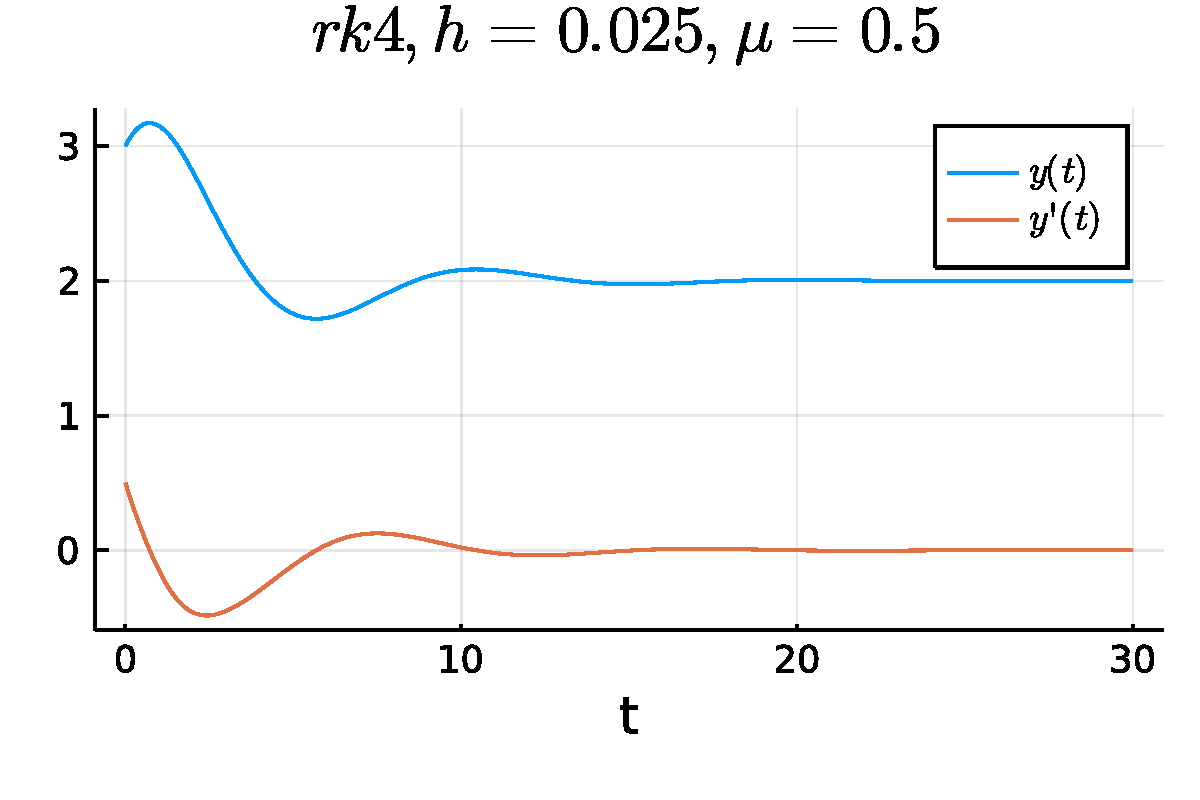
\includegraphics[width=\linewidth]{figures/ass_2_report_2_1.pdf}
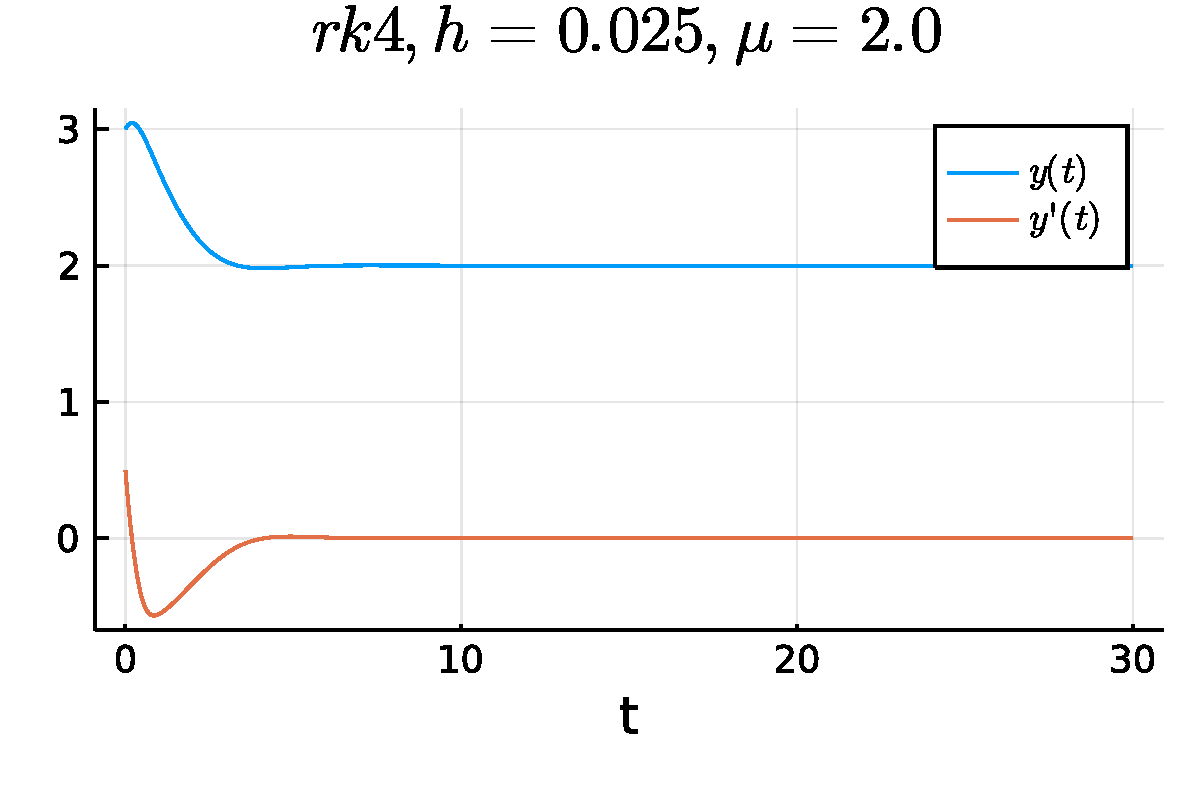
\includegraphics[width=\linewidth]{figures/ass_2_report_2_2.pdf}
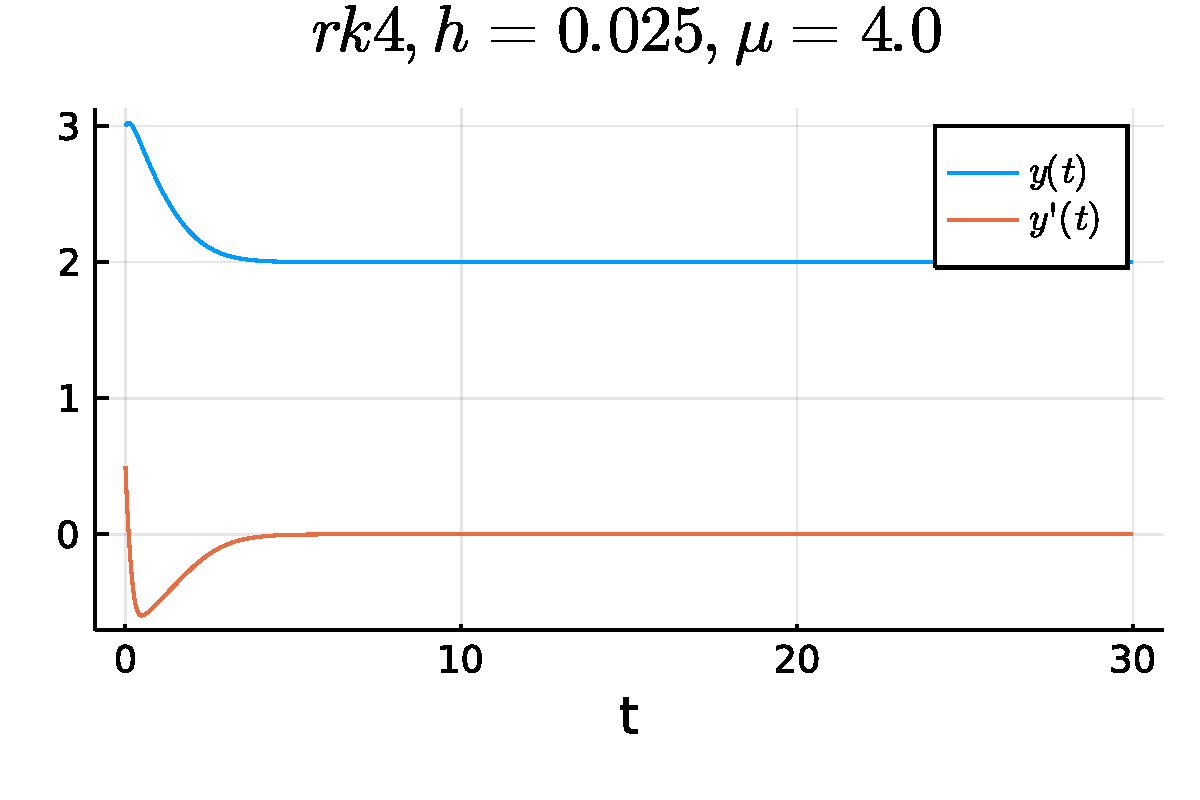
\includegraphics[width=\linewidth]{figures/ass_2_report_2_3.pdf}

\textbf{Plot $y'(t)$ vs $y(t)$}


\begin{lstlisting}
(*@\HLJLk{for}@*) (*@\HLJLn{\ensuremath{\mu}}@*) (*@\HLJLkp{in}@*) (*@\HLJLn{\ensuremath{\mu}s}@*)
    (*@\HLJLn{u}@*) (*@\HLJLoB{=}@*) (*@\HLJLnf{rk4}@*)(*@\HLJLp{(}@*)(*@\HLJLn{func}@*)(*@\HLJLp{,}@*) (*@\HLJLn{N}@*)(*@\HLJLp{,}@*) (*@\HLJLn{T}@*)(*@\HLJLp{,}@*) (*@\HLJLn{u0}@*)(*@\HLJLp{,}@*) (*@\HLJLn{\ensuremath{\mu}}@*)(*@\HLJLp{)}@*)
    (*@\HLJLn{p3}@*) (*@\HLJLoB{=}@*) (*@\HLJLnf{plot}@*)(*@\HLJLp{(}@*)(*@\HLJLn{u}@*)(*@\HLJLp{[}@*)(*@\HLJLni{1}@*)(*@\HLJLp{,}@*)(*@\HLJLoB{:}@*)(*@\HLJLp{],}@*) (*@\HLJLn{u}@*)(*@\HLJLp{[}@*)(*@\HLJLni{2}@*)(*@\HLJLp{,}@*)(*@\HLJLoB{:}@*)(*@\HLJLp{],}@*) (*@\HLJLn{thickness{\_}scaling}@*) (*@\HLJLoB{=}@*) (*@\HLJLnfB{1.5}@*)(*@\HLJLp{,}@*) (*@\HLJLn{legend}@*) (*@\HLJLoB{=}@*) (*@\HLJLkc{false}@*)(*@\HLJLp{)}@*)
    (*@\HLJLnf{xlabel!}@*)(*@\HLJLp{(}@*)(*@\HLJLso{L"{}y(t)"{}}@*)(*@\HLJLp{)}@*)
    (*@\HLJLnf{ylabel!}@*)(*@\HLJLp{(}@*)(*@\HLJLso{L"{}y{\textquotesingle}(t)"{}}@*)(*@\HLJLp{)}@*)
    (*@\HLJLnf{title!}@*)(*@\HLJLp{(}@*)(*@\HLJLnf{latexstring}@*)(*@\HLJLp{(}@*)(*@\HLJLs{"{}rk4,h=0.025,}@*)(*@\HLJLse{{\textbackslash}{\textbackslash}}@*)(*@\HLJLs{mu="{}}@*)(*@\HLJLp{,}@*)(*@\HLJLn{\ensuremath{\mu}}@*)(*@\HLJLp{))}@*)
    (*@\HLJLnf{display}@*)(*@\HLJLp{(}@*)(*@\HLJLn{p3}@*)(*@\HLJLp{)}@*)
(*@\HLJLk{end}@*)
\end{lstlisting}

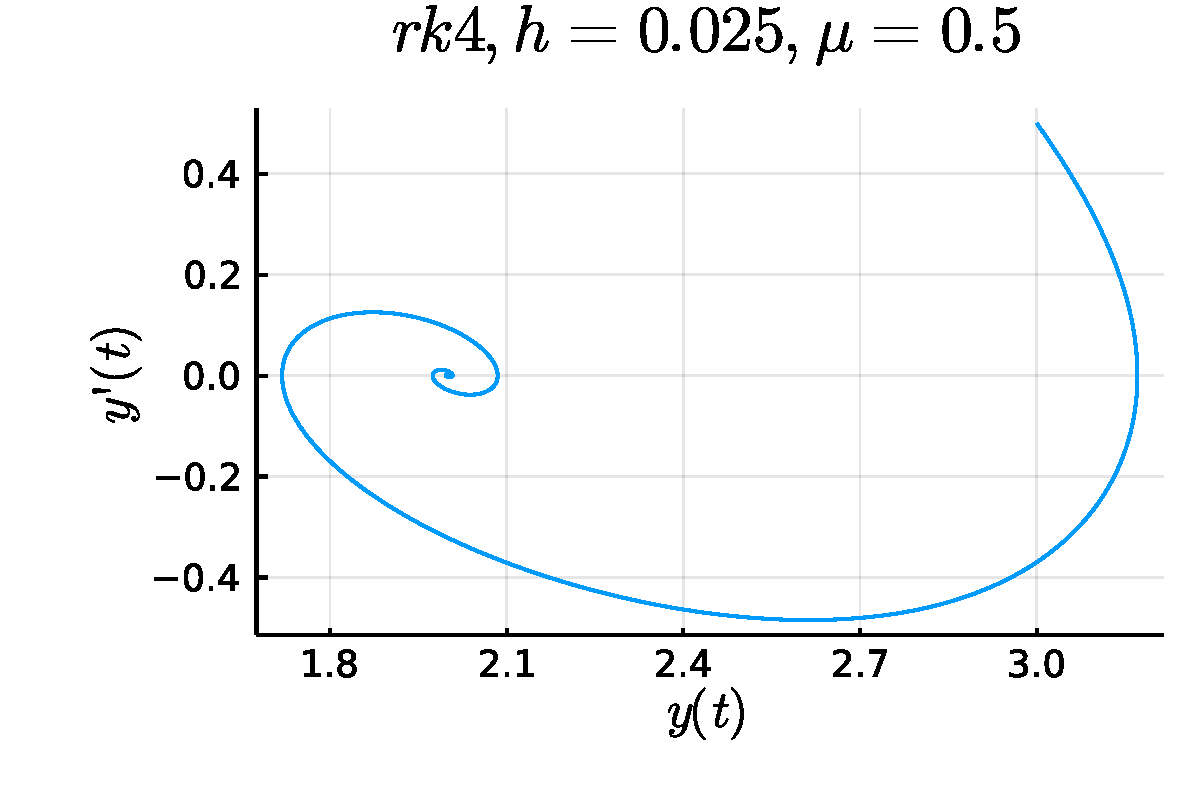
\includegraphics[width=\linewidth]{figures/ass_2_report_3_1.pdf}
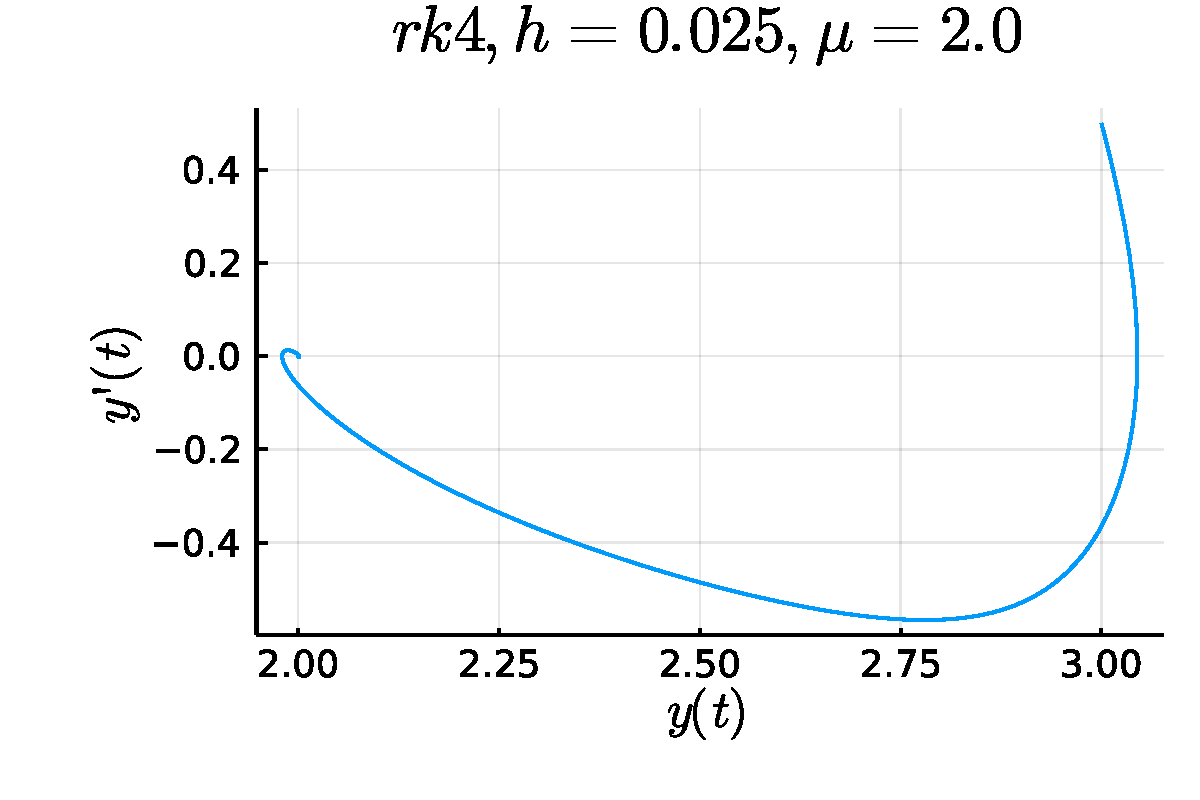
\includegraphics[width=\linewidth]{figures/ass_2_report_3_2.pdf}
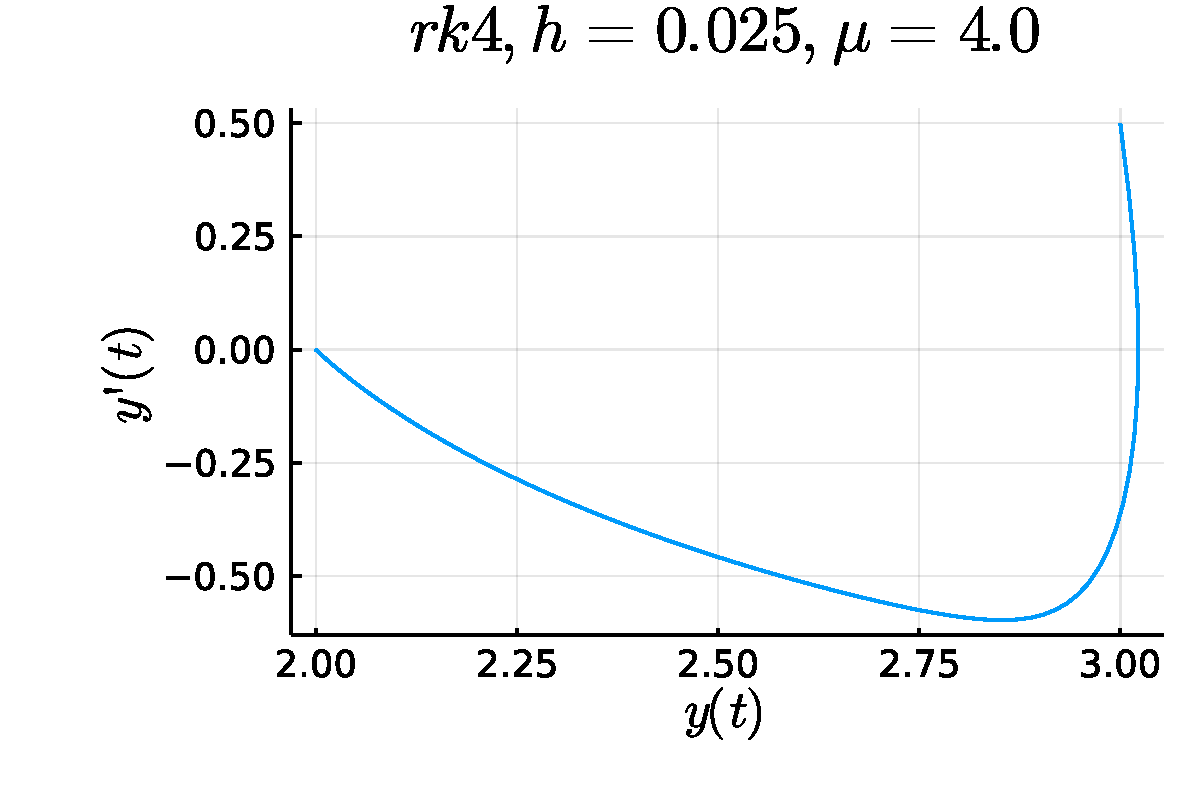
\includegraphics[width=\linewidth]{figures/ass_2_report_3_3.pdf}

\section{Problem 5}
\subsection{Part 1}
Run simulations for decreasing step sizes and plot $E_max$ vs $h$


\begin{lstlisting}
(*@\HLJLcs{{\#}}@*) (*@\HLJLcs{defining}@*) (*@\HLJLcs{variables}@*)
(*@\HLJLn{u0}@*) (*@\HLJLoB{=}@*) (*@\HLJLp{[}@*)(*@\HLJLnfB{3.0}@*)(*@\HLJLp{;}@*) (*@\HLJLnfB{0.5}@*)(*@\HLJLp{]}@*) (*@\HLJLcs{{\#}}@*) (*@\HLJLcs{y(0)}@*) (*@\HLJLcs{and}@*) (*@\HLJLcs{y{\textquotesingle}(0)}@*)
(*@\HLJLn{T}@*) (*@\HLJLoB{=}@*) (*@\HLJLni{30}@*)(*@\HLJLp{;}@*) (*@\HLJLn{\ensuremath{\mu}}@*) (*@\HLJLoB{=}@*) (*@\HLJLnfB{4.0}@*)(*@\HLJLp{;}@*)
(*@\HLJLn{N}@*) (*@\HLJLoB{=}@*) (*@\HLJLnf{Int}@*)(*@\HLJLp{(}@*)(*@\HLJLn{T}@*)(*@\HLJLoB{/}@*)(*@\HLJLn{h}@*)(*@\HLJLp{);}@*)
(*@\HLJLn{t}@*) (*@\HLJLoB{=}@*) (*@\HLJLnf{collect}@*)(*@\HLJLp{(}@*)(*@\HLJLni{0}@*)(*@\HLJLoB{:}@*)(*@\HLJLn{N}@*)(*@\HLJLp{)}@*)(*@\HLJLoB{*}@*)(*@\HLJLn{h}@*)

(*@\HLJLcs{{\#}}@*) (*@\HLJLcs{Part}@*) (*@\HLJLcs{1}@*)
(*@\HLJLn{hs}@*) (*@\HLJLoB{=}@*) (*@\HLJLni{1}@*) (*@\HLJLoB{./}@*)(*@\HLJLp{(}@*)(*@\HLJLnfB{2.0}@*) (*@\HLJLoB{.{\textasciicircum}}@*)(*@\HLJLp{(}@*)(*@\HLJLni{3}@*)(*@\HLJLoB{:}@*)(*@\HLJLni{10}@*)(*@\HLJLp{))}@*)
(*@\HLJLn{E{\_}max}@*) (*@\HLJLoB{=}@*) (*@\HLJLnf{zeros}@*)(*@\HLJLp{(}@*)(*@\HLJLnf{size}@*)(*@\HLJLp{(}@*)(*@\HLJLn{hs}@*)(*@\HLJLp{))}@*)
(*@\HLJLk{for}@*) (*@\HLJLn{i}@*) (*@\HLJLoB{=}@*) (*@\HLJLni{1}@*) (*@\HLJLoB{:}@*) (*@\HLJLnf{length}@*)(*@\HLJLp{(}@*)(*@\HLJLn{hs}@*)(*@\HLJLp{)}@*)
    (*@\HLJLn{N}@*) (*@\HLJLoB{=}@*) (*@\HLJLnf{Int}@*)(*@\HLJLp{(}@*)(*@\HLJLn{T}@*)(*@\HLJLoB{/}@*)(*@\HLJLn{hs}@*)(*@\HLJLp{[}@*)(*@\HLJLn{i}@*)(*@\HLJLp{])}@*)
    (*@\HLJLn{u{\_}nh}@*) (*@\HLJLoB{=}@*) (*@\HLJLnf{rk4}@*)(*@\HLJLp{(}@*)(*@\HLJLn{func}@*)(*@\HLJLp{,}@*) (*@\HLJLn{N}@*)(*@\HLJLp{,}@*) (*@\HLJLn{T}@*)(*@\HLJLp{,}@*) (*@\HLJLn{u0}@*)(*@\HLJLp{,}@*) (*@\HLJLn{\ensuremath{\mu}}@*)(*@\HLJLp{)}@*)
    (*@\HLJLn{u{\_}2nh2}@*) (*@\HLJLoB{=}@*) (*@\HLJLnf{rk4}@*)(*@\HLJLp{(}@*)(*@\HLJLn{func}@*)(*@\HLJLp{,}@*) (*@\HLJLni{2}@*)(*@\HLJLoB{*}@*)(*@\HLJLn{N}@*)(*@\HLJLp{,}@*) (*@\HLJLn{T}@*)(*@\HLJLp{,}@*) (*@\HLJLn{u0}@*)(*@\HLJLp{,}@*) (*@\HLJLn{\ensuremath{\mu}}@*)(*@\HLJLp{)}@*)

    (*@\HLJLcs{{\#}}@*) (*@\HLJLcs{subtract}@*) (*@\HLJLcs{every}@*) (*@\HLJLcs{two}@*) (*@\HLJLcs{from}@*) (*@\HLJLcs{u{\_}2nh2}@*)
    (*@\HLJLn{E{\_}max}@*)(*@\HLJLp{[}@*)(*@\HLJLn{i}@*)(*@\HLJLp{]}@*) (*@\HLJLoB{=}@*) (*@\HLJLnf{maximum}@*)(*@\HLJLp{(}@*)(*@\HLJLn{abs}@*)(*@\HLJLoB{.}@*)(*@\HLJLp{(}@*)(*@\HLJLn{u{\_}nh}@*)(*@\HLJLp{[}@*)(*@\HLJLni{1}@*)(*@\HLJLp{,}@*)(*@\HLJLni{1}@*)(*@\HLJLoB{:}@*)(*@\HLJLn{N}@*)(*@\HLJLp{]}@*) (*@\HLJLoB{-}@*) (*@\HLJLn{u{\_}2nh2}@*)(*@\HLJLp{[}@*)(*@\HLJLni{1}@*)(*@\HLJLp{,}@*)(*@\HLJLni{1}@*)(*@\HLJLoB{:}@*)(*@\HLJLni{2}@*)(*@\HLJLoB{:}@*)(*@\HLJLni{2}@*)(*@\HLJLoB{*}@*)(*@\HLJLn{N}@*)(*@\HLJLp{])}@*)(*@\HLJLoB{./}@*)(*@\HLJLp{(}@*)(*@\HLJLni{1}@*)(*@\HLJLoB{-}@*)(*@\HLJLnfB{0.5}@*)(*@\HLJLoB{{\textasciicircum}}@*)(*@\HLJLni{4}@*)(*@\HLJLp{))}@*)
(*@\HLJLk{end}@*)

(*@\HLJLnf{plot}@*)(*@\HLJLp{(}@*)(*@\HLJLn{hs}@*)(*@\HLJLp{,}@*) (*@\HLJLn{E{\_}max}@*)(*@\HLJLp{,}@*) (*@\HLJLn{label}@*) (*@\HLJLoB{=}@*) (*@\HLJLso{L"{}E{\_}{\{}{\textbackslash}max{\}}"{}}@*)(*@\HLJLp{,}@*) (*@\HLJLn{xaxis}@*) (*@\HLJLoB{=}@*) (*@\HLJLsc{:log}@*)(*@\HLJLp{,}@*) (*@\HLJLn{yaxis}@*) (*@\HLJLoB{=}@*) (*@\HLJLsc{:log}@*)(*@\HLJLp{,}@*) (*@\HLJLn{marker}@*) (*@\HLJLoB{=}@*) (*@\HLJLp{(}@*)(*@\HLJLsc{:square}@*)(*@\HLJLp{,}@*)(*@\HLJLni{5}@*)(*@\HLJLp{),}@*) (*@\HLJLn{add{\_}marker}@*) (*@\HLJLoB{=}@*) (*@\HLJLkc{true}@*)(*@\HLJLp{)}@*)
(*@\HLJLnf{xlabel!}@*)(*@\HLJLp{(}@*)(*@\HLJLso{L"{}h"{}}@*)(*@\HLJLp{)}@*)
(*@\HLJLnf{ylabel!}@*)(*@\HLJLp{(}@*)(*@\HLJLso{L"{}{\textbackslash}max||E{\_}n(h)||"{}}@*)(*@\HLJLp{)}@*)
\end{lstlisting}

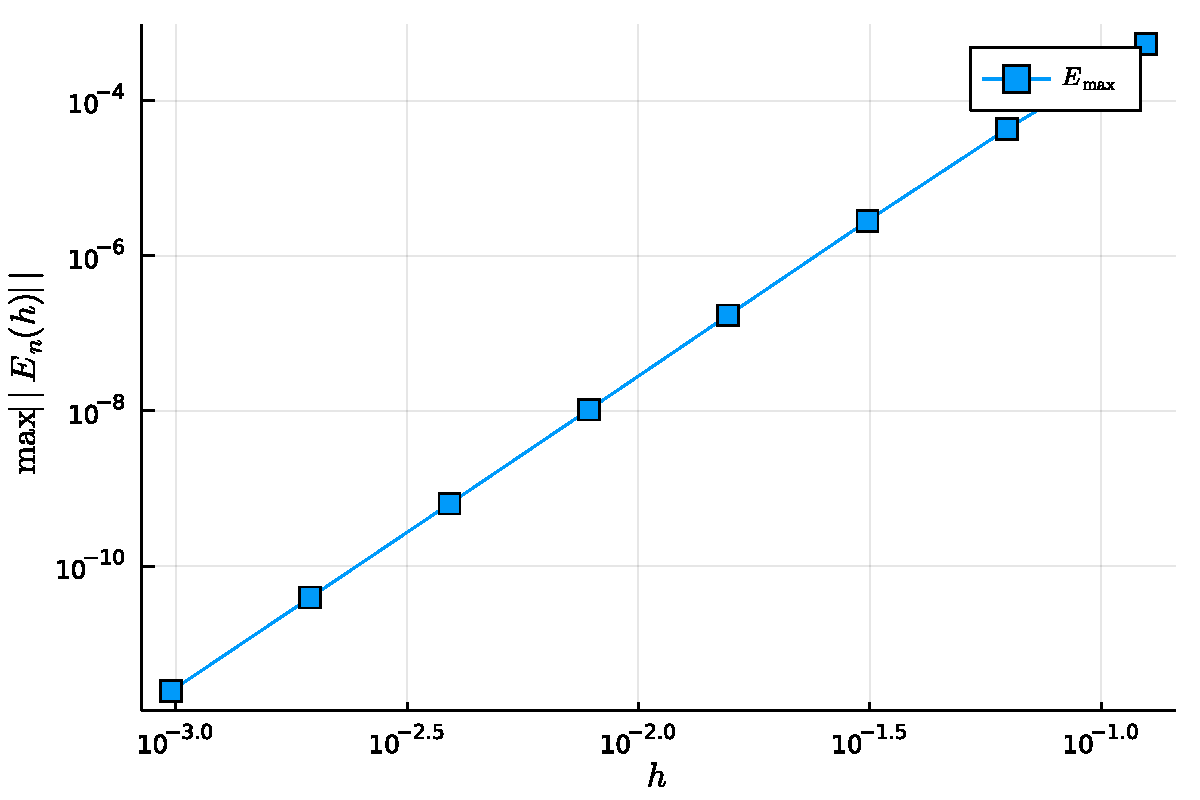
\includegraphics[width=\linewidth]{figures/ass_2_report_4_1.pdf}

Find the value of $h$ where $E_{\max} < 5x10^{-8}$. This occurs at the first index where $E_{\max} < 5x10^{-8}$


\begin{lstlisting}
(*@\HLJLcs{{\#}}@*) (*@\HLJLcs{Part}@*) (*@\HLJLcs{2}@*)
(*@\HLJLcs{{\#}}@*) (*@\HLJLcs{Find}@*) (*@\HLJLcs{index}@*) (*@\HLJLcs{where}@*) (*@\HLJLcs{E{\_}max(h)}@*) (*@\HLJLcs{<}@*) (*@\HLJLcs{5}@*) (*@\HLJLcs{x}@*) (*@\HLJLcs{10{\textasciicircum}-8}@*)
(*@\HLJLn{index}@*) (*@\HLJLoB{=}@*) (*@\HLJLnf{findfirst}@*)(*@\HLJLp{(}@*)(*@\HLJLn{x}@*)(*@\HLJLoB{->}@*)(*@\HLJLn{x}@*) (*@\HLJLoB{<}@*) (*@\HLJLnfB{5.0}@*)(*@\HLJLoB{*}@*)(*@\HLJLp{(}@*)(*@\HLJLnfB{10.0}@*)(*@\HLJLoB{{\textasciicircum}}@*)(*@\HLJLp{(}@*)(*@\HLJLoB{-}@*)(*@\HLJLni{8}@*)(*@\HLJLp{)),}@*) (*@\HLJLn{E{\_}max}@*)(*@\HLJLp{)}@*)
(*@\HLJLn{hs}@*)(*@\HLJLp{[}@*)(*@\HLJLn{index}@*)(*@\HLJLp{]}@*)
\end{lstlisting}

\begin{lstlisting}
0.0078125
\end{lstlisting}


$h = \frac{1}{2^7}$

\section{Problem 6}
\subsection{Part 1}
Plot $E_n^{(Fehlberg)}(h)$ vs $t_n$


\begin{lstlisting}
(*@\HLJLcs{{\#}}@*) (*@\HLJLcs{defining}@*) (*@\HLJLcs{variables}@*)
(*@\HLJLn{u0}@*) (*@\HLJLoB{=}@*) (*@\HLJLp{[}@*)(*@\HLJLnfB{3.0}@*)(*@\HLJLp{;}@*) (*@\HLJLnfB{0.5}@*)(*@\HLJLp{]}@*) (*@\HLJLcs{{\#}}@*) (*@\HLJLcs{y(0)}@*) (*@\HLJLcs{and}@*) (*@\HLJLcs{y{\textquotesingle}(0)}@*)
(*@\HLJLn{T}@*) (*@\HLJLoB{=}@*) (*@\HLJLni{30}@*)(*@\HLJLp{;}@*) (*@\HLJLn{\ensuremath{\mu}}@*) (*@\HLJLoB{=}@*) (*@\HLJLnfB{4.0}@*)(*@\HLJLp{;}@*) (*@\HLJLn{h}@*) (*@\HLJLoB{=}@*) (*@\HLJLnfB{0.025}@*)(*@\HLJLp{;}@*)
(*@\HLJLn{N}@*) (*@\HLJLoB{=}@*) (*@\HLJLnf{Int}@*)(*@\HLJLp{(}@*)(*@\HLJLn{T}@*)(*@\HLJLoB{/}@*)(*@\HLJLn{h}@*)(*@\HLJLp{);}@*)
(*@\HLJLn{t}@*) (*@\HLJLoB{=}@*) (*@\HLJLnf{collect}@*)(*@\HLJLp{(}@*)(*@\HLJLni{0}@*)(*@\HLJLoB{:}@*)(*@\HLJLn{N}@*)(*@\HLJLp{)}@*)(*@\HLJLoB{*}@*)(*@\HLJLn{h}@*)

(*@\HLJLcs{{\#}}@*) (*@\HLJLcs{Part}@*) (*@\HLJLcs{1}@*)
(*@\HLJLp{(}@*)(*@\HLJLn{u}@*)(*@\HLJLp{,}@*) (*@\HLJLn{E\ensuremath{\_n}}@*)(*@\HLJLp{)}@*) (*@\HLJLoB{=}@*) (*@\HLJLnf{fehlberg}@*)(*@\HLJLp{(}@*)(*@\HLJLn{func}@*)(*@\HLJLp{,}@*) (*@\HLJLn{N}@*)(*@\HLJLp{,}@*) (*@\HLJLn{T}@*)(*@\HLJLp{,}@*) (*@\HLJLn{u0}@*)(*@\HLJLp{,}@*) (*@\HLJLn{\ensuremath{\mu}}@*)(*@\HLJLp{)}@*)

(*@\HLJLcs{{\#}}@*) (*@\HLJLcs{E}@*) (*@\HLJLcs{=}@*) (*@\HLJLcs{E\ensuremath{\_n}[E\ensuremath{\_n}}@*) (*@\HLJLcs{.>}@*) (*@\HLJLcs{10.0{\textasciicircum}(-17)]}@*)
(*@\HLJLn{E}@*) (*@\HLJLoB{=}@*) (*@\HLJLn{E\ensuremath{\_n}}@*)(*@\HLJLp{[}@*)(*@\HLJLn{E\ensuremath{\_n}}@*) (*@\HLJLoB{.!=}@*) (*@\HLJLnfB{0.0}@*)(*@\HLJLp{]}@*)
(*@\HLJLnf{plot}@*)(*@\HLJLp{(}@*)(*@\HLJLn{t}@*)(*@\HLJLp{[}@*)(*@\HLJLni{1}@*)(*@\HLJLoB{:}@*)(*@\HLJLnf{length}@*)(*@\HLJLp{(}@*)(*@\HLJLn{E}@*)(*@\HLJLp{)],}@*) (*@\HLJLn{E}@*)(*@\HLJLp{,}@*) (*@\HLJLn{label}@*) (*@\HLJLoB{=}@*) (*@\HLJLso{L"{}E{\textasciicircum}{\{}Fehlberg{\}}{\_}{\{}n{\}}"{}}@*)(*@\HLJLp{,}@*) (*@\HLJLn{yaxis}@*) (*@\HLJLoB{=}@*) (*@\HLJLsc{:log}@*)(*@\HLJLp{)}@*)
(*@\HLJLnf{xlabel!}@*)(*@\HLJLp{(}@*)(*@\HLJLn{L}@*)(*@\HLJLs{"{}t"{}}@*)(*@\HLJLp{)}@*)
\end{lstlisting}

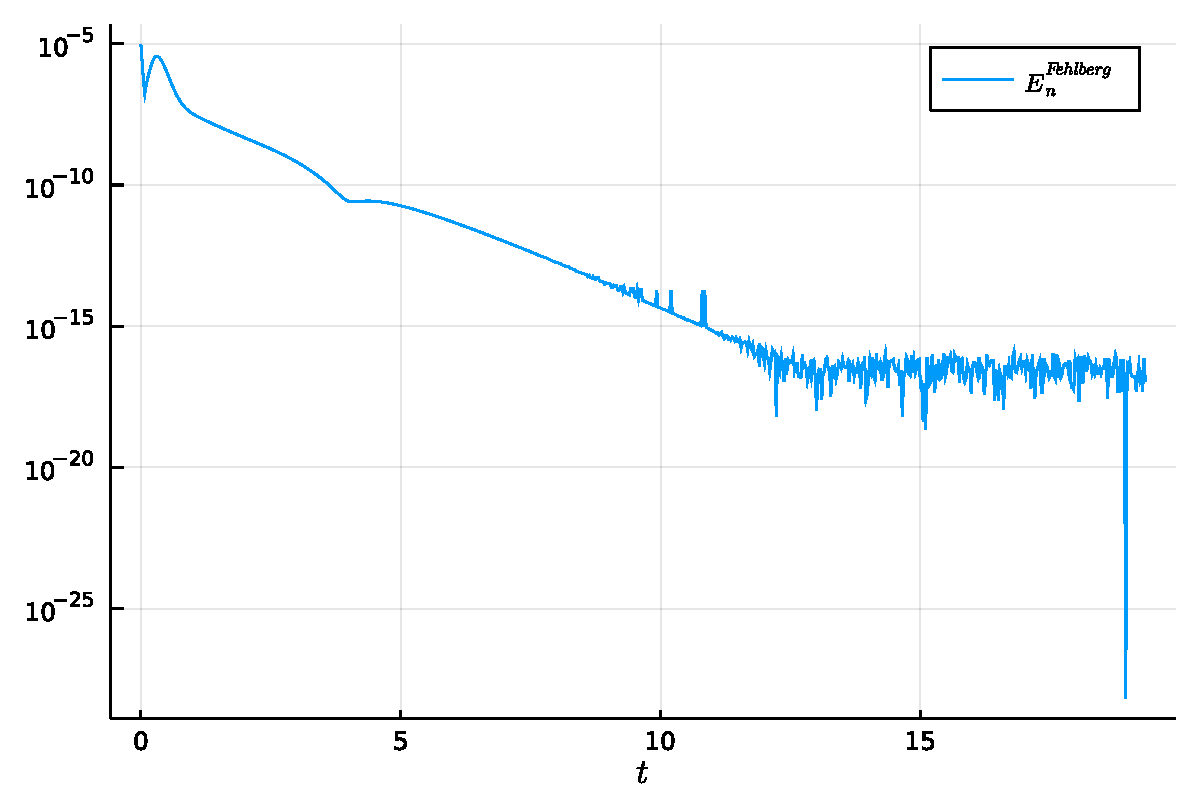
\includegraphics[width=\linewidth]{figures/ass_2_report_6_1.pdf}

\subsection{Part 2}
Plot $E_n$ vs $t_n$


\begin{lstlisting}
(*@\HLJLcs{{\#}}@*) (*@\HLJLcs{Part}@*) (*@\HLJLcs{2}@*)
(*@\HLJLp{(}@*)(*@\HLJLn{u2}@*)(*@\HLJLp{,}@*) (*@\HLJLn{E\ensuremath{\_n}}@*)(*@\HLJLp{)}@*) (*@\HLJLoB{=}@*) (*@\HLJLnf{fehlberg}@*)(*@\HLJLp{(}@*)(*@\HLJLn{func}@*)(*@\HLJLp{,}@*) (*@\HLJLni{2}@*)(*@\HLJLoB{*}@*)(*@\HLJLn{N}@*)(*@\HLJLp{,}@*) (*@\HLJLn{T}@*)(*@\HLJLp{,}@*) (*@\HLJLn{u0}@*)(*@\HLJLp{,}@*) (*@\HLJLn{\ensuremath{\mu}}@*)(*@\HLJLp{)}@*)

(*@\HLJLn{E}@*) (*@\HLJLoB{=}@*) (*@\HLJLn{abs}@*)(*@\HLJLoB{.}@*)(*@\HLJLp{(}@*)(*@\HLJLn{u}@*)(*@\HLJLp{[}@*)(*@\HLJLni{1}@*)(*@\HLJLp{,}@*)(*@\HLJLni{1}@*)(*@\HLJLoB{:}@*)(*@\HLJLn{N}@*)(*@\HLJLp{]}@*) (*@\HLJLoB{-}@*) (*@\HLJLn{u2}@*)(*@\HLJLp{[}@*)(*@\HLJLni{1}@*)(*@\HLJLp{,}@*)(*@\HLJLni{1}@*)(*@\HLJLoB{:}@*)(*@\HLJLni{2}@*)(*@\HLJLoB{:}@*)(*@\HLJLni{2}@*)(*@\HLJLoB{*}@*)(*@\HLJLn{N}@*)(*@\HLJLp{])}@*)(*@\HLJLoB{/}@*)(*@\HLJLp{(}@*)(*@\HLJLni{1}@*)(*@\HLJLoB{-}@*)(*@\HLJLnfB{0.5}@*)(*@\HLJLoB{{\textasciicircum}}@*)(*@\HLJLni{5}@*)(*@\HLJLp{)}@*)
(*@\HLJLn{E}@*) (*@\HLJLoB{=}@*) (*@\HLJLn{E}@*)(*@\HLJLp{[}@*)(*@\HLJLn{E}@*) (*@\HLJLoB{.!=}@*) (*@\HLJLnfB{0.0}@*)(*@\HLJLp{]}@*)
(*@\HLJLnf{plot}@*)(*@\HLJLp{(}@*)(*@\HLJLn{t}@*)(*@\HLJLp{[}@*)(*@\HLJLni{1}@*)(*@\HLJLoB{:}@*)(*@\HLJLnf{length}@*)(*@\HLJLp{(}@*)(*@\HLJLn{E}@*)(*@\HLJLp{)],}@*) (*@\HLJLn{E}@*)(*@\HLJLp{,}@*) (*@\HLJLn{label}@*) (*@\HLJLoB{=}@*) (*@\HLJLso{L"{}E{\_}n"{}}@*)(*@\HLJLp{,}@*) (*@\HLJLn{yaxis}@*) (*@\HLJLoB{=:}@*)(*@\HLJLn{log}@*)(*@\HLJLp{)}@*)
(*@\HLJLnf{xlabel!}@*)(*@\HLJLp{(}@*)(*@\HLJLso{L"{}t"{}}@*)(*@\HLJLp{)}@*)
\end{lstlisting}

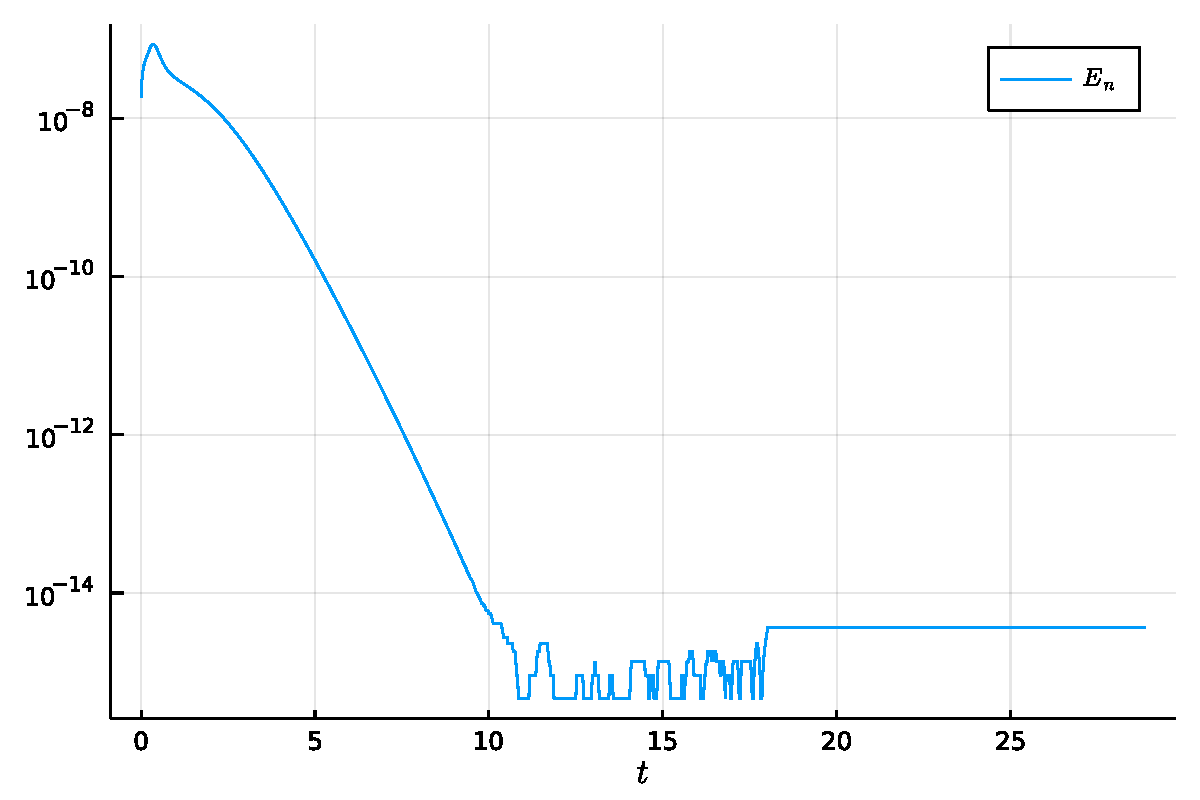
\includegraphics[width=\linewidth]{figures/ass_2_report_7_1.pdf}


\end{document}
